%	
%	disposition.tex
%	
%	This document provides a summary of all of the exam question topics for
%	the algorithms and datastructures course at the university of copenhagen
%	department of computer science. It was written to serve as an excellent
%	asset for the oral exam preparation, with most of the subtopics covered
%	for any given exam topic in a concise and easily understandable format.
%	

\documentclass[11pt,english]{book}

\usepackage{appendix}						% appendices
\usepackage[linesnumbered]{algorithm2e}		% algorithm pseudo-code
\usepackage{amsmath,amssymb}				% mathematical notation
\usepackage{fancyhdr}						% page styling
\usepackage{float}							% for floating figures
\usepackage{sectsty}						% section styling
\usepackage{tikz} 							% for graphs

%========== meta data ==========%

\title
{
	Algorithms \& Datastructures\\
	\huge Disposition
}

\author
{
	Casper B. Hansen\\
	\small Department of Computer Science\\
	\small The University of Copenhagen\\
	\texttt{fvx507@alumni.ku.dk}
% fix this, makes footnote number, and it shouldn't!
%	\thanks{Adam Honoré}
%	\thanks{Mads Torhus}
}


\date{\today}


%========== settings ==========%

\setlength{\headheight}{15pt}
\sectionfont{\Large}


%========== macros ==========%

\newcommand{\sethead}[3]{\lhead{#1}\chead{#2}\rhead{#3}}
\newcommand{\setfeet}[3]{\lfoot{#1}\cfoot{#2}\rfoot{#3}}

%========== document ==========%

\begin{document}

\frontmatter
\maketitle
\thispagestyle{empty}
\tableofcontents

%========== preamble ==========%

\newpage
\pagestyle{fancy}

\chapter*{Preamble}
In this document we will discuss the most important principles of algorithms
and datastructures in accordance with the syllabus of the course under the
same title at the University of Copenhagen, Department of Computer Science.

\section*{About the authors}
We're a small group of Computer Science students, attending the course
mentioned above at the time of writing this document as collaborative effort
to make a great disposition for the course exam, that will both increase our
own understanding of the subjects discussed as well as produce an invaluable
resource for others attending the course, or who wish to learn about
algorithms and datastructures in generel.

\section*{Why we made this document}
The document is was written in order to support our own understanding of the
course contents as well as aid us during the exam preparation time.

\section*{How to use this document}
The intention of the document is \textit{not} to be a fullfledged introduction
to algorithms and datastructure that you can just pick up and start learning
from. As such it requires at least an accompanying book, or that you are
attending lectures on the subject, or some other means that provide a base
knowledge.

The document is merely a tool for looking up things quickly, and defines the
subjects in a concise manner, hence no in-depth discussion of any subject is
to be found in this document. The sole purpose of the document is precisely
that; a resource for quickly looking up the concepts discussed presented at
lectures, or in a book.

\section*{Recommendations}
As far as we know the book \textit{Introduction to Algorithms} by Thomas H.
Cormen, Charles E. Leiserson, Ronald L. Rivest and Clifford Stein, is pretty
much the go-to choice if you want to study algorithms, and since this was our
textbook during the course this is what we'll recommend for you.



\mainmatter
%========== Divide & Conquer ==========%

\chapter{Divide \& Conquer}
\label{ch:divideandconquer}

\textbf{Relevant Assignment} Problem ?-?\\\\
\textbf{Algorithms} Merge sort, quicksort\\\\
\textbf{Keywords} The master method, recursion trees (validation by induction)
\vspace{1in}

\noindent Divide and conquer is paradigm of algorithmic methodologies.
% more?
\\\\
\noindent \textbf{Divide} the problem into a number of subproblems that are
smaller instances of the same problem.
\\\\
\noindent \textbf{Conquer} the subproblems by solving them recursively. If the
subproblem sizes are small enough, however, just solve the subproblems in a
straightforward manner.
\\\\
\noindent \textbf{Combine} the solutions to the subproblems into the solution
for the original problem.
\\\\

\section{Recursion Trees}
A recursion tree is a pictorial representation of an algorithms recursive
calls. That is, we simply draw the recursions as they occur in a
tree-structure, such that we may [...]

Although recursion trees are useful for getting an idea about the complexity
of a recursive algorithm, it doesn't directly give us any concrete about this.
For that must employ more strict methods that are rooted in mathematics, and
not drawings.

\section{Solving Recurrences}
...

\section{Substitution}
...

\section{The Master Method}
...


%========== Heaps ==========%

\chapter{Heaps}
\label{ch:heaps}

\textbf{Relevant Assignment} Problem ?-?\\\\
\textbf{Pensum} CLRS Ch. 6\\\\
\textbf{Keywords} Min- and maxheap, sorting, priority queues
\vspace{1in}

\noindent A heap is a nearly complete $n$-nary tree, we will concern ourselves
only with binary heaps - and as such, a binary heap is a nearly complete
binary tree. A heap implements a set $S$ of elements, in which each element
has an associated key. The actual structure of a heap is simply an array, and
so a heap is defined by the operations performed on the array, rather than the
data structure itself. The reason a heap is a tree-structure is a
visualization of the data, but not reflected by the data structure in any way.

Visualizing the array of a heap as a tree, we have that the root of the tree
corresponds to the first element of the array $i = 0$ (zero-indexed). The
parent of any node $n$ is given by $\lfloor n/2 \rfloor$. The children are
given by $2n$ and $2n + 1$, for left and right, respectively.

\newpage
\noindent Using the rules of traversal defined above, we can visualize the
array
\begin{figure}[H]
	\center
	\begin{tabular}{|c|c|c|c|c|c|c|c|c|c|}
		\hline 16 & 14 & 10 & 8 & 7 & 9 & 3 & 2 & 4 & 1 \\ \hline
	\end{tabular}
	\caption{Example of a (binary-)heap}
	\label{fig:heap-array}
\end{figure}
as a tree-structure, as shown in the following figure.
\begin{figure}[H]
	\center
	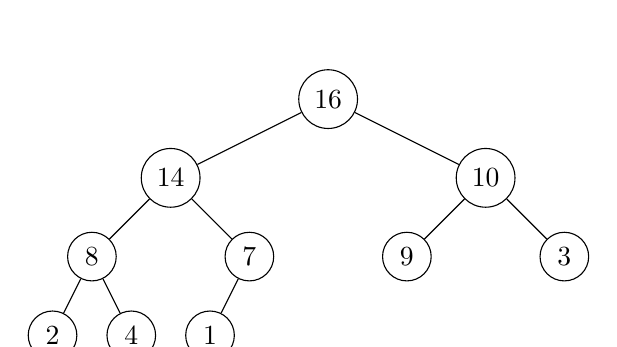
\begin{tikzpicture}
	[
	scale=1.0,
	align=center,
	every node/.style={circle, fill=white, draw=black}
	]
		% level 1
		\node (n1) at 	(3.5, -1) {16};
		
		% level 2
		\node (n2) at 	(1.5, -2) {14};
		\node (n3) at 	(5.5, -2) {10};
		
		% level 3
		\node (n4) at 	(0.5, -3) {8};
		\node (n5) at 	(2.5, -3) {7};
		\node (n6) at 	(4.5, -3) {9};
		\node (n7) at 	(6.5, -3) {3};
		
		% level 4
		\node (n8) at 	(0, -4) {2};
		\node (n9) at 	(1, -4) {4};
		\node (n10) at 	(2, -4) {1};
		% \node (n11) at 	(3, -4) {11};
		% \node (n12) at 	(4, -4) {12};
		% \node (n13) at 	(5, -4) {13};
		% \node (n14) at 	(6, -4) {14};
		% \node (n15) at 	(7, -4) {15};
		
		% drawing code
		\foreach \from/\to in {n1/n2,n1/n3} \draw (\from) -- (\to);
		\foreach \from/\to in {n2/n4,n2/n5,n3/n6,n3/n7} \draw (\from) -- (\to);
		\foreach \from/\to in {n4/n8,n4/n9,n5/n10} \draw (\from) -- (\to);
	\end{tikzpicture}
	\caption{Example of a (binary-)heap visualized as a tree}
	\label{fig:heap-tree}
\end{figure}
...

\section{Priority Queues}
\label{ch:heaps|sub:priorityqueues}
A priority queue is an abstract data structure, which sorts and maintains a
set of data in such a way, that the data is prioritized. It is an important
distinction to make that a priority queue isn't a particular data structure,
but rather a class of data structures. Data structures that work well with
this notion include stacks, heaps, self-organizing lists, etc. We will focus
mainly on heaps.

A heap, however, is not a priority queue in and of itself, it must adhere to
a set of properties, and that is either the max- or min-heap properties.
\begin{description}
	\item \textbf{Max-heap} The key of a node is greater than or equal to the
keys of its children.
	\item \textbf{Min-heap} The key of a node is less than or equal to the
keys of its children.
\end{description}
As the max- and min heaps are defined by the procedures performed on them, we
must show that the their property is maintained by each of these procedures.

\begin{algorithm}[H]
	\caption{Max-heapify algorithm}
	\label{alg:max-heapify}
	
	\SetKwInOut{Input}{Input}
	\SetKwInOut{Output}{Output}
	
	\SetKwFunction{MaxHeapify}{MaxHeapify}
	\SetKwFunction{Left}{Left}
	\SetKwFunction{Right}{Right}
	
	\Input{An array $A$ and index $i$}
	\Output{In-place swapping max-heap property violations of $A$.}
	
	\BlankLine
	\MaxHeapify($A$, $i$) \\
	\Begin
	{
		$l = $ \Left($i$) \\
		$r = $ \Right($i$) \\
		$largest = i$ \\
		\If{$l \leq A.size $ \textnormal{and} $A[l] > A[i]$}
		{
			$largest = l$ \\
		}
		\If{$r \leq A.size $ \textnormal{and} $A[r] > A[largest]$}
		{
			$largest = l$ \\
		}
		\If{$largest \neq i$}
		{
			Swap $A[i]$ and $A[largest]$ \\
			\MaxHeapify($A$, $largest$)
		}
	}
\end{algorithm}
Obviously, this function can easily be changed to \textit{min-heapify}, simply
by exchanging the conditional statements of $\leq$ with $\geq$, and likewise
$>$ to $<$. The procedure looks for a violation of the max-heap property,
restoring it by correcting that particular instance and check for further
violations on the corrected index.

Assuming the worst case, where the subproblem size is $2n/3$ we get the
recurrence $T(n) \leq T(2n/3) + \Theta(1)$, which by the master theorem (see
section \ref{eqn:master-theorem}) gives us $T(n) = O(\lg n)$, which
conveniently translates to the height of a tree - so for a given node $i$, we
at most correct a \textit{simple path} of the tree, or we can visualize it as
the violating node travels only in a downward path.

% possibly shorten the above, making space for explanation of the next
% algorithm, such that maybe we can have it all on one page.

\begin{algorithm}[H]
	\caption{Build max-heap}
	\label{alg:build-max-heap}
	
	\SetKwInOut{Input}{Input}
	\SetKwInOut{Output}{Output}
	
	\SetKwFunction{BuildMaxHeap}{BuildMaxHeap}
	\SetKwFunction{MaxHeapify}{MaxHeapify}
	
	\SetKw{DownTo}{ down to }
	
	\Input{An array $A$}
	\Output{In-place heapifying the array $A$.}
	
	\BlankLine
	\BuildMaxHeap($A$) \\
	\Begin
	{
		$A.size = A.length$ \\
		\For{$i = \lfloor A.length/2 \rfloor \DownTo 1$}
		{
			\MaxHeapify($A$, $i$)
		}
	}
\end{algorithm}
% pseudo-code for building a *-heap, along with explanation for these.

\section{Procedures}
These are the procedures that are supported by max- or min-heaps.

\subsection{Insertion}
...

% TODO: pseudo-code, complexity

\subsection{Extraction}
When we want to extract an element out of a heap, because of its practical use
we are typically interested only in the root node. Getting the root node is a
trivial problem, we simply return the element at index zero - for a max-heap,
this would be the element with the largest key in the set, vice versa for a
min-heap.

% TODO: pseudo-code, complexity

\subsection{Increase key}
...

% TODO: pseudo-code, complexity

% TODO: prove that all procedures maintain the max- or min-heap property


%========== Balanced Binary Search Trees ==========%

\chapter{Balanced Binary Search Trees}
\label{ch:balancedbinarysearchtrees}

\textbf{Relevant Assignment} Problem 13-3\\\\
\textbf{Pensum}CLRS Ch. 12 + 13\\\\
\textbf{Algorithms} Red-black binary trees\\\\
\textbf{Keywords} ...
\vspace{1in}

\noindent ...


%========== Dynamic Programming ==========%

\chapter{Dynamic Programming}
\label{ch:dynamicprog}

\textbf{Relevant Assignment} Week 3, Problem 15-2\\\\
\textbf{Keywords} Rod-cutting, fibonacci, time-memory trade-off
\vspace{1in}

\noindent There are two key characteristics that a problem must have for
dynamic programming to be a viable solution; optimal substructure and
overlapping subproblems.
\\\\
\noindent \textbf{Optimal Substructure}\\
% p. 379
...
\\\\
\noindent \textbf{Overlapping Subproblems}\\
% p. 384 - TODO: make this more concise
When a recursive algorithm revisits the same problem repeatedly, we say that
the optimization problem has \textit{overlapping subproblems}. That is, we
solve the same subproblems, rather than generating new subproblems. In
contrast to the divide and conquer technique, where we generate and solve new
subproblems that are smaller instances of the same type of problem, in dynamic
programming we solve each subproblem once, and then storing the solution in a
table, where it can be looked up when needed in $\Theta(1)$ time.

\newpage
\section{Discovering Optimal Substructure}
% p. 379-380
\begin{enumerate}
	\item Show that a solution to the problem consists of making a choice.
Making this choice leaves one or more subproblems to be solved.
	\item Suppose that for a given problem there exists a choice which leads
to an optimal substructure. Do not concern yourself with how to determine this
choice, but assume it has been given to you.
	\item Given this choice, determine which subproblems ensue and how to best
characterize the resulting space of subproblems.
	\item Using a "cut-and-paste" technique, show that the solutions to the
subproblems must themselves be optimal. You can do so by supposing that each
subproblem is not optimal and then deriving a contradiction.

The "cut-and-paste" refers to cutting out the nonoptimal solution for each of
the subproblems, and pasting in the optimal one. Doing so shows that for the
original problems solution to be optimal, so must its subproblems.

Should an optimal solution give rise to more than one subproblem, they are
typically so similar that you can modify the cut-and-paste argument for one to
apply to the others with little effort.
\end{enumerate}

\newpage
\section{Methods of Approach}
There are usually two equivalent ways to implement a dynamic-programming
approach; top-down with memoization and bottom-up.

\subsection{Top-down with Memoization}
% taken directly from the CLRS book, good summary I think.
In this approach, we write the procedure recursively in a natural manner, but
modified to save the result of each subproblem (usually in an array or hash
table). The procedure now first checks to see whether it has previously solved
this problem. If so, it returns the saved value, saving further computation at
this level; if not, the procedure computes the value in the usual manner. We
say that the recursive procedure has been \textit{memoized}; it "remembers"
what results it has computed previously.

\subsection{Bottom-up}
% taken directly from the CLRS book, good summary I think.
This approach typically depends on some natural notion of the "size" of a
subproblem, such that solving any particular subproblem depends only on
solving "smaller" subproblems.

We sort the subproblems by size and solve them in size order, smallest first.
When solving a particular subproblem, we have already solved all of the
smaller subproblems its solution depends upon, and we saved their solutions.
We solve each subproblem only once, and when we first see it, we have already
solved all of its prerequisite subproblems.

\newpage
\section{Running Time Analysis}
% p. 380-381
...


%========== Greedy Algorithms ==========%

\chapter{Greedy Algorithms}
\label{ch:greedyalgorithms}

\textbf{Pensum} 16 \cite{clrs} \\\\
\textbf{Assignments} 16-1 \\\\
\textbf{Algorithms} Activity selection, huffman trees \\\\
\textbf{Keywords} The greedy choice, local- and global optimal solution
\vspace{1in}

\noindent Greedy algorithms follow an algorithmic methodology that makes a
series of choices under the assumption that the choice that seems best at the
moment (a \textit{locally optimal solution}) will produce \textit{globally
optimal solution} - this isn't always the case, but in some cases we can prove
that it does.
\\\\
\noindent \textbf{Dynamic Programming} \\
Although greedy problems often exhibit the same characteristics as a dynamic
programming problem, the key difference between these two algorithmic
techniques is that dynamic programming problems tries all possible solutions,
and hence always yields an optimal solution. This is not necessarily the case
for a greedy algorithm, as it does not concern itself with the subproblem, but
rather makes a locally optimal choice \textit{in the hope} that this will lead
to a globally optimal solution - we can, however, show that it will for some
problems.

\newpage
\section{The Greedy Strategy}
Here we list the procedure one must follow in order to design a greedy
algorithm. Each point will be discussed in depth under its own section.
\begin{enumerate}
	\item \textbf{Describe} the optimization problem as one in which making a
choice, we are left with one subproblem.
	\item \textbf{Prove} that the greedy choice always yields a globally
optimal solution.
	\item \textbf{Demonstrate} optimal substructure by showing that, having
made a greedy choice, what remains is a subproblem with the property that if
we combine an optimal solution with the greedy greedy choice, we arrive at an
optimal solution to the original problem.
\end{enumerate}

\subsection{Describing the Optimization Problem}
% p. ?-?, CLRS
...

\subsection{Proving The Greedy Choice}
% p. 424, CLRS
As the greedy choice is not always the optimal choice, you will have to prove
the choice for each algorithme. The proof examines a globally optimal solution
to some subproblem. It then shows how to modify the solution to substitute the
greedy choice for some other choice, resulting in one similar, but smaller,
subproblem.

\subsection{Demonstrating Optimal Substructure}
% p. ?-?, CLRS
...

\clearpage
\section{Huffman Codes}
% p. 428-435, CLRS
The Huffman code algorithm compresses data by constructing a tree-structure
from the data by means of the frequency of occurrences within the data.
\\\\
\begin{algorithm}[H]
	\SetKwInOut{In}{Input}
	\SetKwInOut{Out}{Output}
	
	\SetKwFunction{HuffmanCode}{HuffmanCode}
	\SetKwFunction{ExtractMin}{ExtractMin}
	\SetKwFunction{Insert}{Insert}
	
	\In{A data set $C$, each node within it has an attribute $freq$.}
	\Out{The root node of the tree-structure built.}
	\BlankLine
	
	\HuffmanCode($C$) \\
	\Begin
	{
		$n = |C|$ \\
		$Q = C$ \\
		\For{$i = 1$ \KwTo $n - 1$}
		{
			allocate a new node $z$ \\
			$z.left = x = $ \ExtractMin($Q$) \\
			$z.right = y = $ \ExtractMin($Q$) \\
			$z.freq = z = x.freq + y.freq$ \\
			\Insert($Q$, $z$)
		}
		\Return \ExtractMin($Q$)
	}
\end{algorithm}

\subsection{Analysis}
During the initialization it sets $n$ to the cardinality of the set $C$ on
line 3, and builds a min-heap priority queue from the set $C$, keyed on the
frequency of the nodes, on line 4. The latter taking the majority of the
running-time of the initialization at $O(n)$ (see algorithm
\ref{alg:build-max-heap} on page ~\ref{alg:build-max-heap}).

The loop in lines 5--11 runs exactly $n-1$ times, executing heap operations
that take $O(\lg n)$ each, and so it contributes a total of $O(n \lg n)$.

% \subsection{Proof}
% We must first show that the problem exhibits optimal substructure, and that
% the greedy choice is always right. First we show that the greedy choice holds.

% \begin{lemma}
	
% \end{lemma}


%========== Amortized Complexity ==========%

\chapter{Amortized Complexity}
\label{ch:amortizedcomplexity}

\textbf{Relevant Assignment} Week ?, Problem ?-?\\\\
\textbf{Keywords} Aggregate analysis, accounting- and potential method, average.
\vspace{1in}

\noindent In amortized complexity analysis, we average the time required to
perform a sequence of data-structure operations over all the operations
performed. With amortized analysis, we can show that the average cost of an
operation is small, if we average over a sequence of operations, even though
a single operation within the sequence might be expensive.
\\\\
\noindent \textbf{Amortized- and Average-case Analysis} \\
Amortized analysis differs from average-case analysis in that probability is
not involved; an amortized analysis guarantees the \textit{average performance
of each operation in the worst case}.

\newpage
\section{Aggregate Analysis}
In aggregate analysis, we show that for all $n$, a sequence of $n$ operations
takes \textit{worst-case} time $T(n)$ in total. The average cost, or \textbf{
amortized cost}, however, per operation is $\frac{T(n)}{n}$. The amortized
cost applies to each operation, even when there are several types of
operations in the sequence.

\subsection{Example}
...

\section{Accounting Method}
In the accounting method of amortized complexity analysis, we \textit{assign}
a cost to each operation - this amortized cost does not necessarily reflect
the actual cost of an operation. When an operation's amortized cost exceeds
its actual cost, we perceive this as deposited credit that we can use to pay
for subsequent operations that might be undercharged, that is an operation
whose amortized cost is less than its actual cost.

Although this method is very similar to \textit{aggregate analysis}, the key
difference between these is that in aggregate analysis all operations have
the same amortized cost, whereas in the accounting method we may assign
different amortized cost for different operations.

It follows naturally in aggregate analysis that the total amortized cost of
$n$ operations provides an upper bound on the total actual cost of the
sequence, but for the accounting method we must define this explicitly.
\begin{align}
	\sum_{i=1}^{n}{\hat{c_i}} \geq \sum_{i=1}^{n}{c_i}
	\quad \text{, where }c_i\text{ is the actual cost, and }
	\hat{c_i}\text{ is the amortized cost.}
\end{align}
This relationship, as described by the above equation, must hold for all
sequences of operations.

\subsection{Example}
...

\section{Potential Method}
...

\subsection{Example}
...


%========== Minimum Spanning Trees ==========%

\chapter{Minimum Spanning Trees}
\label{ch:minimumspanningtrees}

\textbf{Pensum} 23 \cite{clrs} \\\\
\textbf{Assignments} 13-3 \\\\
\textbf{Algorithms} Kruskal's, Prim's\\\\
\textbf{Keywords} Greedy, optimal substructure, representation invariant,
binary- and fibonacci-heap
\vspace{1in}

\noindent A minimum spanning tree $T$ is a is a tree or graph whose edges are
a subset $T \subseteq E$ of a weighted graph $G = (V, E)$, with weight
function $w$, such that the weight of an edge $(u, v) \in E$ is determined by
$w$, and the weight of the tree $T$ is minimized.

The total weight of a graph $T$ is given by the sum of all of its edge weights.
\begin{align}
	w(T) = \sum_{(u, v) \in T}w(u, v)
\end{align}

The term \textit{spanning} refers to the fact that the tree $T$ spans the
entire set of vertices $V$, and the term \textit{minimum} refers to that the
tree $T$ is of minimum weight.

\section{Optimal Substructure}
...

\section{Overlapping Subproblems}
...
% TODO: prove that removing an edge (u, v) yields two separate trees.

\newpage
\section{Generic Minimum Spanning Tree}
% p. 626, CLRS
The algorithm given below for finding the minimum spanning tree is a
generalization, meaning that it is somewhat loosely defined. As such, this
is merely a template for building an actual algorithm.
\begin{algorithm}
	\SetKwInOut{Input}{Input}
	\SetKwInOut{Output}{Output}
	
	\SetKwFunction{GenericMST}{GenericMST}
	
	\Input{A graph $G = (V, E)$ and a weight function $w$ defined on $E$.}
	\Output{A minimum spanning tree of $G$.}
	
	\BlankLine
	
	\GenericMST($G$, $w$) \\
	\Begin
	{
		$A = \emptyset$ \\
		\While{$A$ \textnormal{does not form a spanning tree}}
		{
			find an edge $(u, v)$ that is safe for $A$ \\
			$A = A \cup \{(u, v)\}$
		}
	}
	
	\caption{GenericMST}
	\label{alg:generic-mst}
\end{algorithm}
\subsection{Loop Invariant}
We state the loop invariant of algorithm \ref{alg:generic-mst}; prior to each
iteration, $A$ is a subset of some minimum spanning tree.
\\\\
\noindent \textbf{Initialization} \\
After line 3, where we initialize the set $A$ to the empty set, $A$ trivially
satisfies the loop invariant, as the empty set is a subset of any set.
\\\\
\noindent \textbf{Maintenance} \\
Lines 4-7 maintains the loop invariant, because we only add \textit{safe}
edges to $A$. That is, edges $(u, v)$ where $A \cup \{(u, v)\}$ also
satisfies the loop invariant.
\\\\
\noindent \textbf{Termination} \\
Since all edges added to $A$ are in a minimum spanning tree, $A$ must be a
minimum spanning tree of $G$.

\newpage
\section{Kruskal's Algorithm}
% p. 631
...

% TODO: pseudo-code

\newpage
\section{Prim's Algorithm}
% p. 634
This algorithm relies on a priority queue (see section
\ref{ch:heaps|sub:priorityqueues} on page \pageref{ch:heaps|sub:priorityqueues}
for more on this topic).
\\\\
\begin{algorithm}[H]
	\caption{Prim's algorithm}
	\label{alg:prim-mst}
	
	\SetKwInOut{Input}{Input}
	\SetKwInOut{Output}{Output}
	
	\SetKwFunction{PrimMST}{PrimMST}
	\SetKwFunction{ExtractMin}{ExtractMin}
	
	\SetKw{Nil}{NIL}
	
	\Input{A graph $G$, a weight function $w$ and an arbitrary root $r$.}
	\Output{In-place minimized spanning tree of $G$.}
	
	\BlankLine
	\PrimMST($G$, $w$, $r$) \\
	\Begin
	{
		% initialization O(V)
		\For{$u \in G.V$}
		{
			$u.key = \infty$ \\
			$u.\pi = $ \Nil
		}
		$r.key = 0$ \\
		$Q = G.V$ \\
		
		% ... O(?)
		\While{$Q \neq \emptyset$}
		{
			$u = \ExtractMin(Q)$ \\
			\For{$v \in G.Adj[u]$}
			{
				\If{$v \in Q$ \textnormal{and} $w(u, v) < v.key$}
				{
					$v.\pi = u$ \\
					$v.key = w(u, v)$
				}
			}
		}
	}
\end{algorithm}
If we relate it to algorithm \ref{alg:generic-mst} we see that for Prim's
algorithm the exit condition of forming a spanning tree takes the form of
emptying a priority queue.


%========== Shortest Paths Algorithms ==========%

\chapter{Shortest Paths Algorithms}
\label{ch:shortestpathsalgorithms}

\textbf{Relevant Assignment} Week ?, Problem ?-?\\\\
\textbf{Algorithms} Single-source, Dijkstra, Bellman-Ford\\\\
\textbf{Keywords} ...
\vspace{1in}

\noindent Unlike 



\appendix
%========== Asymptotic Notation ==========%

\thispagestyle{fancyplain}

\chapter{Asymptotic Notation}
\label{ch:asymptoticnotation}
The analysis of the growth of a function is called asymptotic analysis. The
mathematical notation used to describe this analysis is called asymptotic
notation.

\section{$O$}
\label{ch:asymptoticnotation|sec:big-o}
Defines a tight upperbounded growth of a function. That is, $O(n)$ is
analogous to the comparison $\leq$.

\section{$o$}
\label{ch:asymptoticnotation|sec:little-o}
...

\section{$\Omega$}
\label{ch:asymptoticnotation|sec:big-omega}
...

\section{$\omega$}
\label{ch:asymptoticnotation|sec:litte-omega}
...

\section{$\Theta$}
\label{ch:asymptoticnotation|sec:theta}
...


%========== Proving Algorithms ==========%

\thispagestyle{fancyplain}

\chapter{Proving Algorithms}
\label{ch:proofs}

In this appendix section we give common techniques shared by many, if not all,
algorithmic paradigms.

\section{Loop Invariant}
\label{ch:proofs|sec:loop-invariant}
A loop invariant is based on the notion of mathematical induction, as it
provides a proof of the algorithms correctness in all three of its executed
stages; initialization, maintenance and termination.

The loop invariant is used to prove the correctness of a loop-based algorithm,
and as such we must make sure that when we state a loop invariant the
following is true.
\\\\
\textbf{Initialization}
\label{ch:proofs|sec:loop-invariant|sub:initialization}\\
The loop invariant is true prior to the first iteration of the loop.
\\\\
\textbf{Maintenance}
\label{ch:proofs|sec:loop-invariant|sub:maintenance}\\
If it is true before an iteration of the loop, it remains true before the next
iteration.
\\\\
\textbf{Termination}
\label{ch:proofs|sec:loop-invariant|sub:termination}\\
When the loop terminates, the invariant provides a useful property that helps
to show that the algorithm is correct.


%========== Useful Equations ==========%

\thispagestyle{fancyplain}

\chapter{Useful Equations}
\label{appendix:equations}
In this appendix section we give the most relevant equations, that are used
throughout the document.

\section{The Triangle Inequality}
\label{appendix:equations|eqn:triangle-inequality}
The triangle inequality states that any two sides combined length of any
triangle always exceeds that of the remaining side.
\begin{align}
	z < x + y
\end{align}

\section{Arithmetic Series}
\label{appendix:equations|eqn:arithmetic-series}
An arithmetic series is a sum of the members of a finite arithmetic
progression.
\begin{align}
	a_1 + a_2 + \dots + a_n = \sum_{i=1}^{n}a_i = \frac{n(a_1 + a_n)}{2}
\end{align}

\section{Telescoping Sums}
\label{appendix:equations|eqn:telescoping}
A sum in which subsequent terms cancel each other, leaving only the first and
the last.
\begin{align}
	S &= \sum_{i=1}^{n-1}(a_{i} - a_{i+1}) \\
	&= (a_1-a_2)+(a_2-a_3) + \dots + (a_{n-2}-a{n-1}) + (a_{n-1}-a_n)
	\nonumber \\
	&= (a_1 - a_n) \nonumber
\end{align}

\section{Integrating and Differentiating series}
\label{appendix:equations|eqn:intdiff-series}
By integrating or differentiating infinite geometric series and multiplying by
$x$, we get
\begin{align}
	\sum_{k=0}^{\infty} kx^k = \frac{x}{(1 - x)^2}
	\quad \text{, for } |x| < 1 \text{.}
\end{align}



\backmatter
%========== bibliography ==========%

\newpage

\sethead{}{Bibliography}{}

\begin{thebibliography}{9}
\label{bibliography}

\bibitem{clrs}
  Thomas H. Cormen, Charles E. Leiserson, Ronald L. Rivest, Clifford Stein\\
  \textit{Introduction to Algorithms}\\
  MIT Press, 3rd. Edition, 2009\\

\end{thebibliography}



\end{document}

